\section{Hologramm}

Ein Hologramm ist in gewissem Sinne die Weiterentwicklung des Photos. Während bei einem Schwarzweißfilm nur die Intensität 
des Wellenfeldes gemessen wird, misst ein Farbphoto schon die Wellenlänge des verwendeten Lichtes mit. Das Hologramm 
beinhaltet nun außerdem Informationen über die Phase des Lichtes. Damit lässt sich ein dreidimensionales Abbild des 
Objektes rekonstruieren. Dabei wird das Hologramm mit einer bestimmten Quelle, der Referenzquelle, aufgenommen. Will man diese nun wiedergeben, benötigt man 
die Referenzquelle oder eine gleichartige Quelle. Wir haben hier ein Hologramm untersucht. Dieses zeigt einen Schlumpf 
beim Fußballspielen, was man in Abbildung \ref{bild:Holo} bewundern kann. 

\begin{figure}[ht]
    \centering
    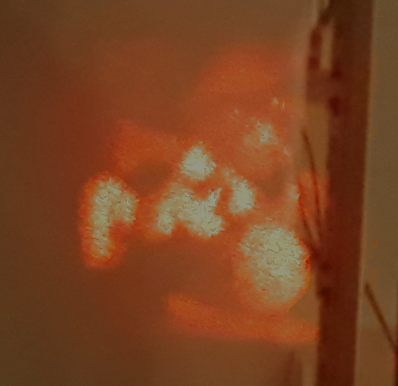
\includegraphics[width = 12cm]{Bilder/Auswertung/Holo.png}
    \caption{Hologramm mit einem HeNe-Hilfslaser aufgenommen}
    \label{bild:Holo}
\end{figure}

Dabei ist das Hologramm leider nicht optimal zu sehen, da wir nur den Hilfslaser verwenden konnten. Trotzdem sieht
man auch in Abbildung \ref{bild:Holo} die dreidimensionale Darstellung des Bildes.